\documentclass[preprint,12pt]{elsarticle}

\usepackage{hyperref}
\usepackage{graphicx}
\usepackage{subcaption}
\usepackage{amssymb}
\usepackage{amsmath}
\usepackage{multirow}
\usepackage{booktabs}
\usepackage[utf8]{inputenc}
\usepackage{cleveref}
\usepackage[section]{placeins}

% For the TODOs
\usepackage{xcolor}
\usepackage{xargs}
\usepackage[colorinlistoftodos,textsize=footnotesize]{todonotes}
\newcommand{\todoin}{\todo[inline]}
% from here: https://tex.stackexchange.com/questions/9796/how-to-add-todo-notes
\newcommandx{\unsure}[2][1=]{\todo[linecolor=red,backgroundcolor=red!25,bordercolor=red,#1]{#2}}
\newcommandx{\change}[2][1=]{\todo[linecolor=blue,backgroundcolor=blue!25,bordercolor=blue,#1]{#2}}
\newcommandx{\info}[2][1=]{\todo[linecolor=OliveGreen,backgroundcolor=OliveGreen!25,bordercolor=OliveGreen,#1]{#2}}

%Boldtype for greek symbols
\newcommand{\teng}[1]{\ensuremath{\boldsymbol{#1}}}
\newcommand{\ten}[1]{\ensuremath{\mathbf{#1}}}

\usepackage{lineno}


\journal{}

\begin{document}

\begin{frontmatter}

  \title{Fluid structure interaction with ETVF}
  \author[IITB]{A Dinesh\corref{cor1}}
  \ead{adepu.dinesh.a@gmail.com}
  \author[IITB]{Prabhu Ramachandran}
  \ead{prabhu@aero.iitb.ac.in}
  \address[IITB]{Department of Aerospace Engineering, Indian Institute of
    Technology Bombay, Powai, Mumbai 400076}

\cortext[cor1]{Corresponding author}

\begin{abstract}
\end{abstract}

\begin{keyword}
%% keywords here, in the form: keyword \sep keyword
{XXX}, {XXX}, {XXX}

%% MSC codes here, in the form: \MSC code \sep code
%% or \MSC[2008] code \sep code (2000 is the default)

\end{keyword}

\end{frontmatter}

% \linenumbers



\section{Introduction}
\label{sec:intro}

Some FSI introduction. Its importance in different fields. Its applications so
far.


In modelling FSI problems, there are mainly two ways to handle the fluid and
structures modelling. One way is to model the fluid part with mesh based
scheme and solids part also with mesh based scheme. Like how (cite many papers
which have done this). Or fluid part is modelled with a particle based scheme
and the structures part with a mesh based scheme (Cite articles which have
done this). One more way is to model both the phases using particle based
schemes. In this paper we use particle based method to model both the phases.


Recently there has been very good work on modelling fsi with particle based
methods. Specific to particle based modelling, the fluid is modelled with SPH,
and structure is modelled with different numerical method. Few articles which
have done in this regard are as follows, citet{hosseini2009particle} has
modelled the structure part using EBG method, then \citet{wu2016coupled}
modelled it with DEM, \citet{ng2020coupled} modeled it using volume
compensated particle method (VCPM), \citet{peng2021coupling} modeled it with
RKPM, citet{zhang2021deltasph} modeled it with Smoothed Point Interpolation
Method (SPIM).


Recently there have been heavy improvements to basic SPH methodology in
modelling fluid problems. Schemes such as $\delta$ SPH, $\delta +$ SPH, TVF
for internal flows and GTVF for external flows is been proposed. Also, many
new strategies were proposed to in overcoming the particle homogeneity
problem, such as IPST, which is applied in \cite{IPST paper}. Also these
improvements take care of tensile instability problem too. Another variant of
SPH is ISPH, todoin{please cite some ISPH papers here}.


Using only SPH, articles have been proposed where we model both the phases
only using SPH. To note some, \citet{He2017coupled} has modelled the fluid
part with WCSPH, \citet{Sun2019study} with delta sph,
\citet{zhan2019stabilized} with WCSPH but applied to 3d problems with GPU. All
these schemes use TLSPH as to model the structure part. And papers by Abbas use
usual Gray equations to model the structures part.

\citet{sun2019fully} couples MPS and BPM model to simulate FSI. He models both
elastic dam break and flow over an elastic obstacle.



Recently {cite our paper ETVF} has been proposed as an another extension to
TVF to model both fluid and structures part. In the current work we couple
purely Eulerian SPH based schemes to model the FSI problems. We take advantage
of the accuracy of the ETVF scheme proposed in modelling the fluids. ETVF
scheme deals with tensile instability in both fluid and solid inherently.




\section{Governing equations}


\subsection{Discrete governing equations}

In this current paper the fluid medium is modelled using the improvised scheme
of TVF, which is been applied to the free surface flows, called ETVF.

For detailed derivation we point the reader to paper \cite{cite our paper},
here we only give the discrete equations.


The discretized equations of the fluid medium are

\begin{equation}
  \label{eq:sph-discretization-continuity}
  \frac{\tilde{d}\rho_a}{dt} = \sum_{b} \; \frac{m_b}{\rho_{b}} \; (
  \rho_{a} \; \tilde{\ten{u}}_{ab} \; + \;
  (\rho \; (\tilde{\ten{u}} \; - \;
  \ten{u}))_{ab}) \; \cdot \nabla_{a} W_{ab},
\end{equation}

\begin{multline}
  \label{eq:sph-discretization-edac}
  \frac{\tilde{d}p_a}{dt} = \sum_{b} \; \frac{m_b}{\rho_{b}} \; \bigg(
  (p_{a} - \rho_{a} c_{s}^2) \; \ten{u}_{ab} \; - \;
  p_{a} \; \tilde{\ten{u}}_{ab} \; - \;
  (p \; (\tilde{\ten{u}} - \ten{u}))_{ab} \; + \; \\
  4 \; \nu_{edac}
  \frac{p_a - p_b}{(\rho_a + \rho_b) (r^2_{ab} + EPS)} \ten{r}_{ab}
  \bigg) \; \cdot \nabla_{a} W_{ab}
\end{multline}


\begin{multline}
  \label{eq:sph-momentum-fluid}
  \frac{\tilde{d}\ten{u}_{a}}{dt} = - \sum_{b} m_b \bigg[
  \bigg(\frac{p_a}{\rho_a^2} + \frac{p_b}{\rho_b^2}\bigg) \ten{I} -
  \bigg(\frac{\ten{A}_a}{\rho_a^2} + \frac{\ten{A}_b}{\rho_b^2}\bigg) \bigg]
  \nabla_{a} W_{ab} \\
  + \ten{u}_{a} \sum_{b} \frac{m_b}{\rho_{b}} \; \tilde{\ten{u}}_{ab} \cdot \nabla_{a} W_{ab} +
  \ten{g}_{a}.
\end{multline}


\begin{equation}
  \label{eq:sph-momentum-solid}
  \frac{\tilde{d}\ten{u}_{a}}{dt} = - \sum_{b} m_b \bigg[
  \bigg(\frac{p_a}{\rho_a^2} + \frac{p_b}{\rho_b^2}\bigg) \ten{I} -
  \bigg(\frac{\teng{\sigma}^{'}_{a}}{\rho_a^2} +
  \frac{\teng{\sigma}^{'}_{b}}{\rho_b^2}\bigg) \bigg]  \nabla_{a} W_{ab} +
  \ten{g}_{a}.
\end{equation}

The Jaumann's formulation for Hooke's stress provides us with the rate of
change of deviatoric stress,
\begin{equation}
  \label{eq:jaumann-stress-rate}
  \frac{d \sigma'_{ij}}{dt} = 2G (\dot{\epsilon}_{ij} - \frac{1}{3}
  \dot{\epsilon}_{ij} \delta_{ij}) + \sigma^{'}_{ik}  \Omega_{jk} +
  \Omega_{ik} \sigma^{'}_{kj}
\end{equation}
where $G$ is the shear modulus, $\dot{\epsilon}_{ij}$ is the strain rate tensor,
\begin{equation}
  \label{eq:strain-tensor}
  \dot{\epsilon}_{ij} = \frac{1}{2} \bigg(\frac{\partial u_i}{\partial x_j} +
  \frac{\partial u_j}{\partial x_i} \bigg)
\end{equation}
and $\Omega_{ij}$ is the rotational tensor,
\begin{equation}
  \label{eq:rotational-tensor}
  \Omega_{ij} = \frac{1}{2} \bigg(\frac{\partial u_i}{\partial x_j} -
  \frac{\partial u_j}{\partial x_i} \bigg)
\end{equation}

\begin{equation}
  \label{eq:sph-vel-grad}
  \nabla \ten{u}_a =
  - \sum_{b} \frac{m_b}{\rho_{b}} (\ten{u}_{a} - \ten{u}_{b}) \otimes (\nabla_{a} W_{ab}),
\end{equation}


In both fluid and solid modelling, the pressure is computed using an
isothermal equation of state, given as,
\begin{equation}
  \label{eq:pressure-equation}
  p = K \bigg(\frac{\rho}{\rho_{0}} - 1 \bigg),
\end{equation}
where $K = \rho_{0} c_0^2$ is the bulk modulus. Here, the constants $c_0$ and
$\rho_0$ are the reference speed of sound and density, respectively.


\subsection{Boundary conditions}


\subsection{Time integration}


\subsection{Coupling between fluid and solid}
\label{subsec:fsi-coupling}

Coupling is handled straight forwardly in SPH. While modelling the fluid phase
and treating the fluid-structure interactions, the structure particles are
assumed to be boundary particles. And from the boundary handling given in
Adami [14], we compute the pressure of the boundary particles from the
extrapolated equation (12) and correspondingly set its density using equation
(13). Please note that the pressure we set here are only pertaining to the fsi
force and does not correspond to the real pressure or density of the structure
particles.

The force acting on the fluid particles is now computed from the pressure set
using the adami boundary conditions and density set consequently. We mark
particles comprising the solid as $a$ and fluid as $i$, and the force acting
on the fluid particle $i$ is given as

\begin{equation}
  f_i^s = -m_i \sum_{a} m_a \bigg(\frac{p_i}{\rho_{i}^2} +
  \frac{p_a}{\rho_{a}^2} + \Pi_{ia} \bigg) \nabla_{i} W(x_{ia})
\end{equation}

Force on the structure particle due to the fluid particle computed using
Newton's third law. Since each structure particle experiences equal and
opposite force as experienced by the fluid particle, the expression for the
force on structure due to a fluid particle is

\begin{equation}
  f_a^F = -m_i \sum_{a} m_a \bigg(\frac{p_a}{\rho_{a}^2} +
  \frac{p_i}{\rho_{i}^2} + \Pi_{ai} \bigg) \nabla_{a} W(x_{ai})
\end{equation}


One more way of coupling is by using \citet{khayyer2018enhanced} formulation.



\subsection{Total energy of the structure}
\label{sec:total-energy-struct}

\citet{khayyer2018enhanced} had an extra section where he discusses about the
energy conservation properties of the proposed FSI scheme. He discusses
different energies in structure, kinetic energy and strain energy.



\section{Results and discussion}
\label{sec:results}

We can get many simple to advanced benchmarks in this area by looking at
applied ocean engineering, coastal engineering, journal of fluids and
structures, marine structures and ocean engineering papers.


The papers we have followed for the benchmarks are
\citet{sun2021accurate}, \citet{yang2016numerical}, \citet{Sun2019study},
\citet{He2017coupled}, \citet{khayyer2018enhanced}, \citet{sun2015numerical},
\citet{wang2020scale}, \citet{peng2021coupling}, \citet{zhang2021deltasph},
\citet{zhan2019stabilized}, \citet{khayyer2021multi},
\citet{long2021coupling}, \citet{ng2020coupled},


% =========================================
% =========================================
% start
% =========================================
% =========================================
\subsection{Hwang 2014 static cantilever beam}
\label{sec:hwang-2014-static-cantilever-beam}
Currently this is a sub problem of elastic dam break. In that problem we are
simulating gate with out considering the gravity. By considering the gravity
we get float division error. It will be interesting to see why such thing is
happening only in the case with gravity and solving such is fun.


\subsection{Dynamics response of an elastic plate}
\label{sec:elastic-plate}

In this example we validate the ETVF scheme in modeling an elastic structure.
This example is taken from \cite{Sun2019study}, who took it from Turek and
Hron, who simulated it using FEM.

An elastic plate is attached to a rigid cylinder. The material properties of
the elastic plate are as follows, the Young's modulus is $1.4\times10^6Pa$ and
a Poisson ratio of $0.4$ and the density is $1000 kg/m^3$. This plate is held
free in a gravity field whose value is $2m/s^2$.


Here we simulate a high speed elastic aluminum wedge impacting on undisturbed
water surface. This benchmark was dealt in
{A $\delta$ SPH-SPIM coupled method for fluid-structure interaction problems} and
{abbas khayyer} papers.
This is an attractive benchmark as it has an semi-analytical solution.

A fluid of length 6 m and a height of 2.2 m is settled inside a tank of length
6m and height 4m which gives rise to a pressure distribution of a hydrostatic
tank. Into this hydrostatic tank a wedge of length 0.6m and a thickness of
0.04m is been dropped with a velocity of 30 m/s. The wedge angle is 10
degrees. Please see figure \ref{fig:half-wedge-deformable} for visual clarity.

The initial particle spacing is set as 0.005m and the total number of
particles combining the wedge, tank and fluid is TOBEDONE. The density of the
fluid is taken as 1000 $kg/m^3$. The material properties of the wedge are as
follows: density of 2700 $Kg/m^3$, Young's modulus of 6.75 1e10 $N/m^2$ and a
Poisson ratio of 0.34. An artificial viscosity $alpha$ of 0.1 is used for
fluids and 1 for solid phase.

In figure \ref{wedge-entering-the-tank}, at different time stamps, we plot the
pressure fields of water and sigma 00 if the flexible wedge. (We need to give
some physical insight of what is expected and what is been observed, provided
our simulations are correct)



A total of three points are marked on the wedge for a qualitative validation.
In figure \ref{point-A-wedge-displacement}, we plot the displacement of point
A with time, and compared with Abbhas and and the semi analytical solution of
scolon 2004. Similarly at point B and point C we compare the pressure of the
current scheme with the one provided with Abbas and the semi analytical
solution. It can be seen that the current scheme is able to produce the
results with a reasonable accuracy.



\subsection{Ng 2020 Hydrostatic water column on an elastic plate}
\label{sec:hydrostatic-water-column-on-an-composite-elastic-plate}

This has two simulations, one taken from \cite{ng2020coupled} and \cite{khayyer2021coupled}.
\begin{table}[!ht]
  \centering
  \begin{tabular}[!ht]{ll}
    % \toprule
    Quantity & Values \\
    % \midrule
    $D$, Diameter & 2m \\
    $\rho_0$, reference density & 1000kg/m\textsuperscript{3} \\
    $c_s$ & 10m/s \\
    $D/\Delta x_{\max}$, lowest resolution & 4 \\
    $D/\Delta x_{\min} $, highest resolution & 160, 250, 500\\
    $C_r$ & 1.08 \\
    Reynolds number & 40, 550, 1000, 3000, and 9500 \\
    Time of simulation & 6 \\
    % \bottomrule
  \end{tabular}
  \caption{Parameters used for the flow past a circular cylinder problem.}%
  \label{tab:fpc-params}
\end{table}
%
%
%
\begin{figure}[!htpb]
  \centering
  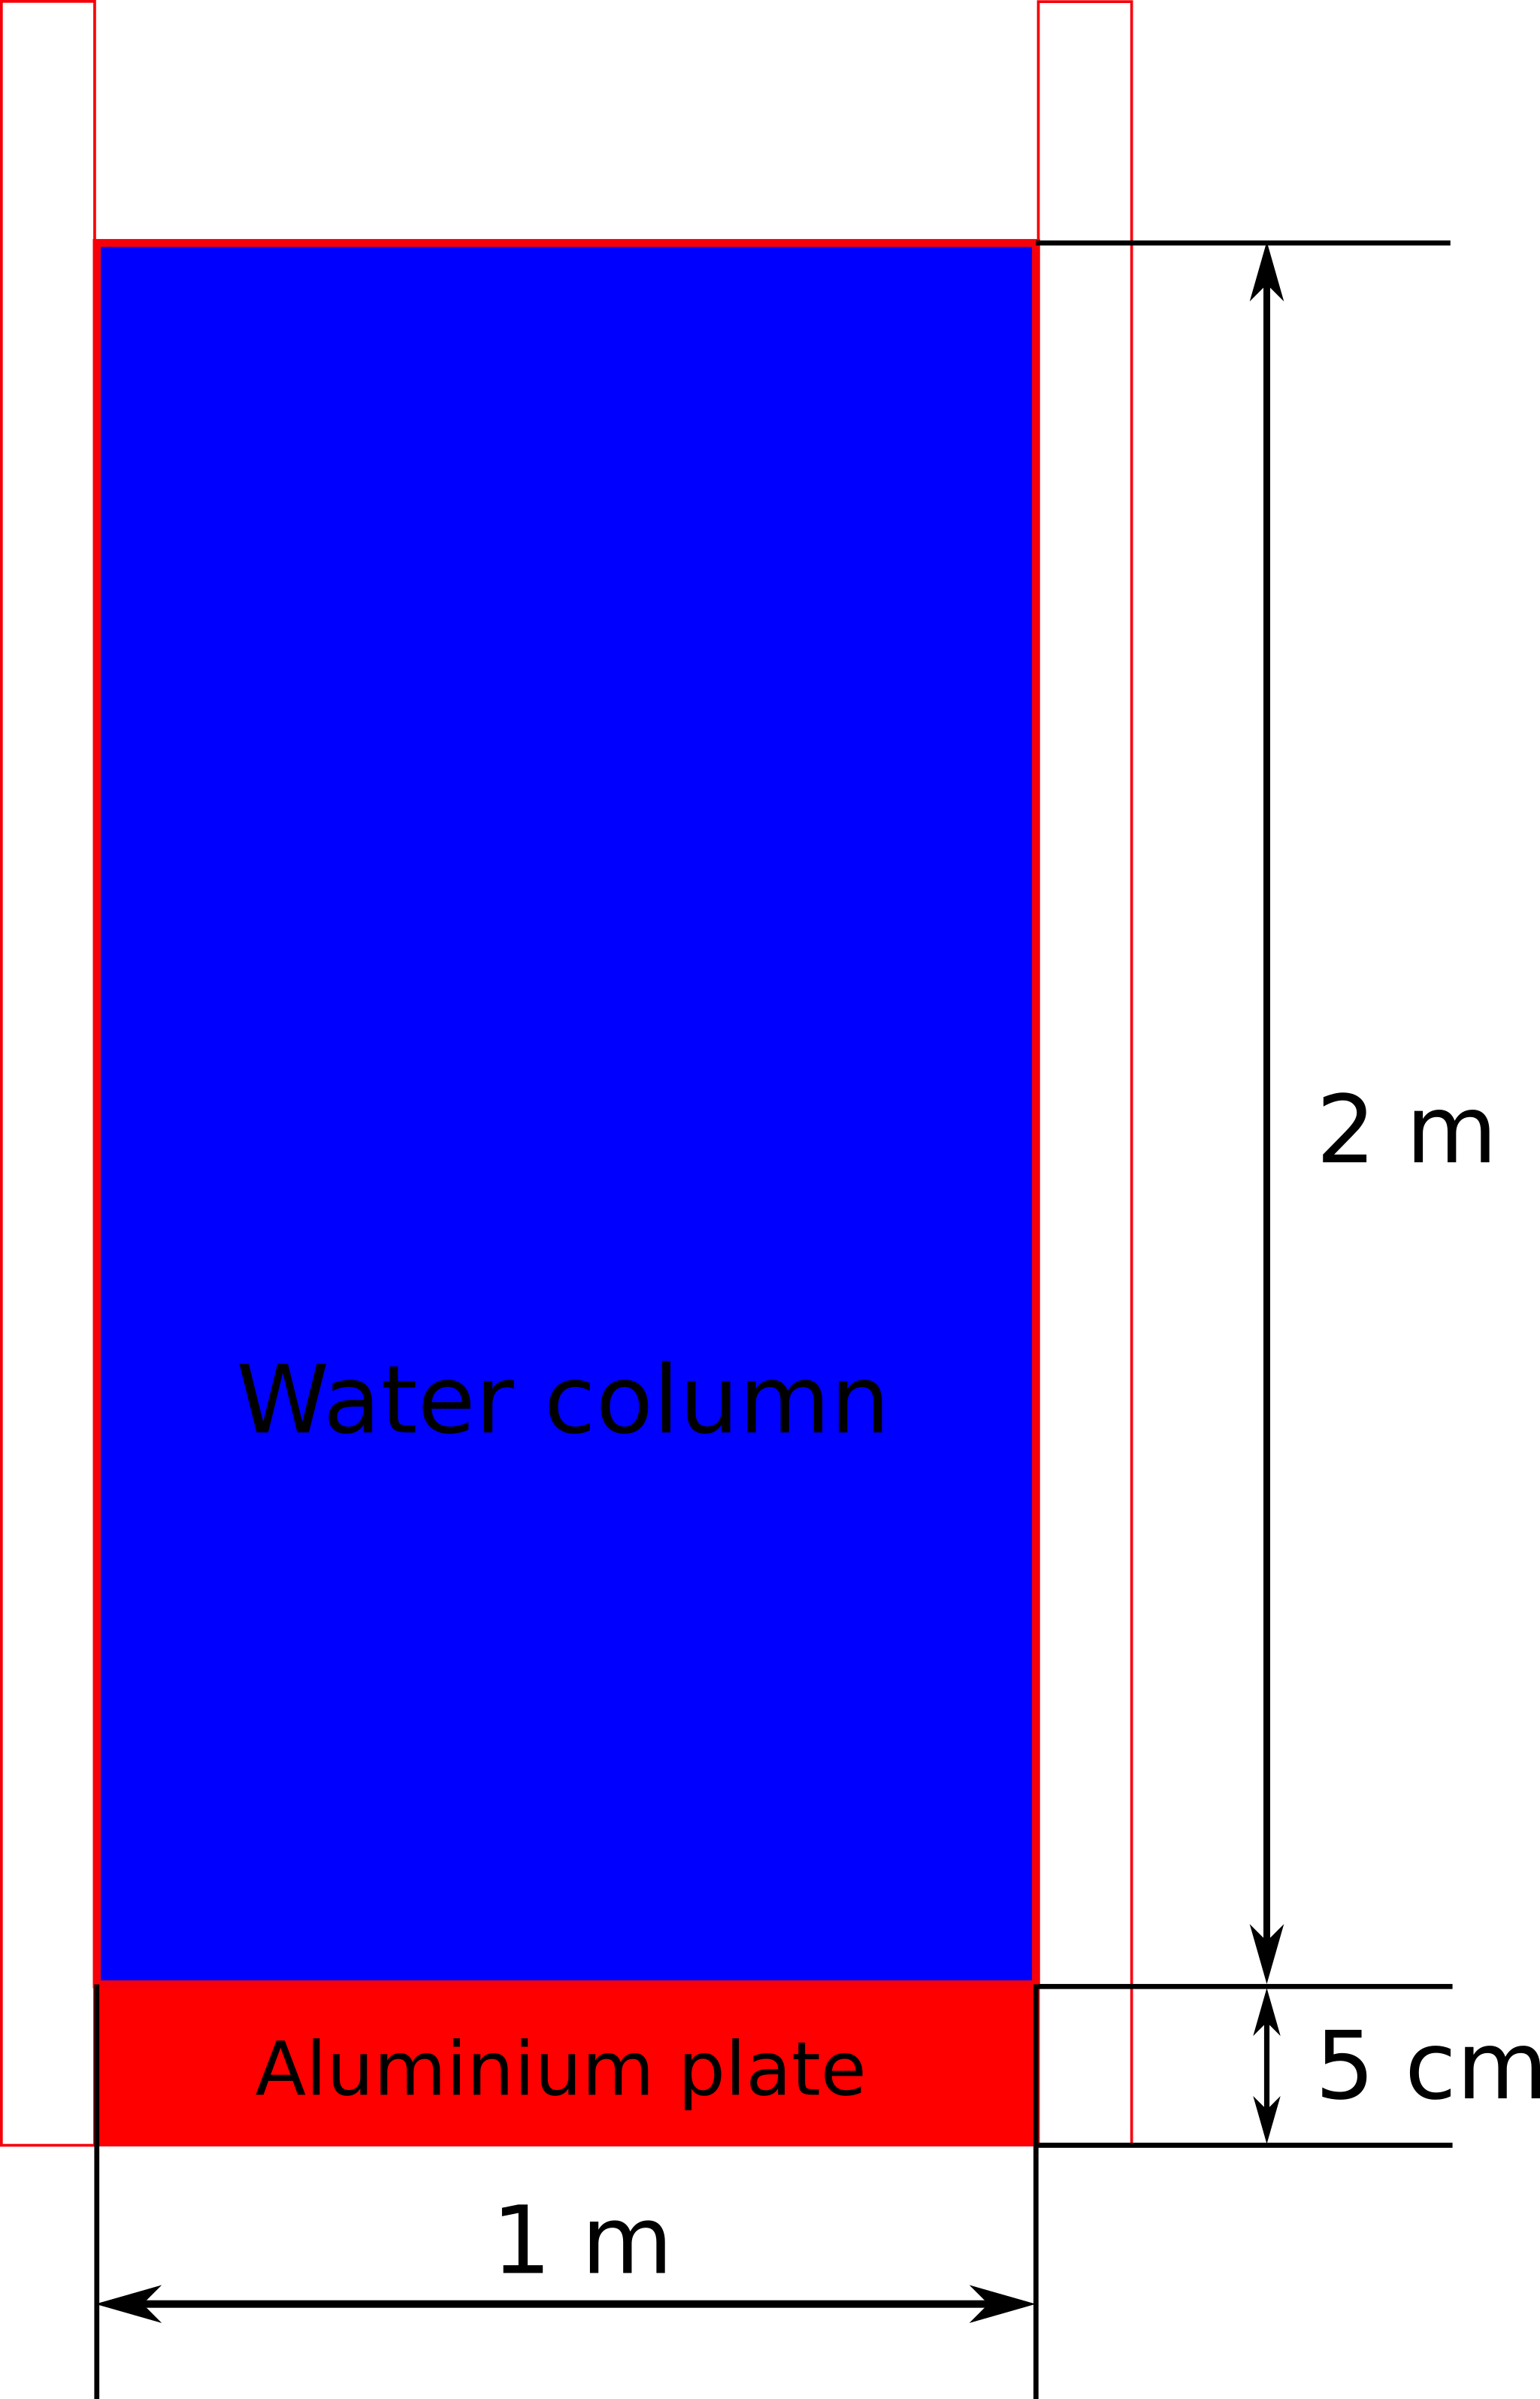
\includegraphics[width=0.4\textwidth]{images/hydrostatic_water_column_on_an_elastic_plate/hydrostatic_water_column_on_an_elastic_plate}
  \caption{Hydrostatic tank}
\label{fig:hs-water-on-plate}
\end{figure}
%
%


\todoin{Comment on the Poisson ratio range of the current scheme}
\todoin{Who did it previously}
\todoin{How to derive the analytical solution in short}
\todoin{Write about the different resolutions}
\todoin{Any other artificial parameters regarding the scheme, alpha, beta}

\todoin{In this problem we check the accuracy and stability-preserving property of the
proposed scheme in handling the fluid structure interaction. This problem has
been studied in Li et al. (2015), Fourey et al. (2017), Khayyer et
al. (2018a), Hu et al. (2019), (2021), (2021) papers. This benchmark has an
analytical solution derived in Li et al. (2015).}


The first benchmark test to validate the fluid structure interaction model
corresponds to an elastic plate under a hydrostatic water tank. An elastic
plate of length 1m and width of 5cm is placed under a block of water column of
height 2m is allowed to settle under gravity. The elastic plate is fixed on
both the ends. The material properties of the water are as follows, the
density is 1000 $kg/m^3$, viscosity of $1e-6$. And the material properties of
the elastic plate are as follows, density 2700$kg/m^3$, Young's modulus
$67.5 \times 10^7$ Pa and a Poisson ratio of 0.34. Three different particle
spacing are considered. Initially the fluid is set up with a hydrostatic
pressure distribution as in equation,
%
%
\begin{equation}
  f_a^F = -m_i \sum_{a} m_a \bigg(\frac{p_a}{\rho_{a}^2} +
  \frac{p_i}{\rho_{i}^2} + \Pi_{ai} \bigg) \nabla_{a} W(x_{ai}).
\end{equation}
%
%
Once the plate reaches an equilibrium state, the
deflection at the midpoint is compared with the analytical solution,
%
%
\begin{equation}
  f_a^F = -m_i \sum_{a} m_a \bigg(\frac{p_a}{\rho_{a}^2} +
  \frac{p_i}{\rho_{i}^2} + \Pi_{ai} \bigg) \nabla_{a} W(x_{ai}).
\end{equation}
%
%
%
\begin{figure}[!htpb]
  \centering
  \includegraphics[width=1\textwidth]{figures/khayyer_2021_hydrostatic_water_column_on_composite_elastic_plate/y_amplitude}
  \caption{Hydrostatic tank}
\label{fig:y-disp-hs-water-on-plate}
\end{figure}
%
%
\Cref{fig:y-disp-hs-water-on-plate} depicts the time histories of the plate's
center point deflection with three different particle spacing. From the
presented \Cref{fig:y-disp-hs-water-on-plate} and table \todoin{citetable} we
can see as the particle spacing is reduced the numerical solution by the
current model approaches the analytical model, which proves the convergence
properties of the current scheme. \todoin{compare with other numerical schemes}
%
%
%
\begin{figure}[!htpb]
  \centering
  \includegraphics[width=1\textwidth]{figures/khayyer_2021_hydrostatic_water_column_on_composite_elastic_plate/y_amplitude}
  \caption{Hydrostatic tank}
\label{fig:p-hs-tank-elastic-plate}
\end{figure}
%
%
%
\begin{figure}[!htpb]
  \centering
  \includegraphics[width=1\textwidth]{figures/khayyer_2021_hydrostatic_water_column_on_composite_elastic_plate/y_amplitude}
  \caption{Hydrostatic tank}
\label{fig:sigma-hs-tank-elastic-plate}
\end{figure}

\Cref{fig:p-hs-tank-elastic-plate} shows the pressure distribution in the
fluid domain at different time histories. \Cref{fig:sigma-hs-water-on-plate}
shows the plots of $\sigma_{00}$ distribution of the elastic plate at
different time steps.

\FloatBarrier%

\subsection{Dam break with elastic gate}
\label{sec:dam-break-elastic-gate}

Taken from \citet{sun2019fully, ng2020coupled}.

A block of fluid, which is suddenly released under gravity hits an elastic
plate. This benchmark is simulated in many papers.

The material properties of the elastic gate are as follows, and Young's
modulus of $0.01 GPa$ with a Poisson ratio of $0.35$ and a density of
$2500 kg/m^3$.

The length of the fluid block is taken as $0.1m$, and the height is $0.3m$,
and the length of the elastic gate is $0.03m$ with a height of $0.05m$ and is
placed at a distance of $0.1m$ from the end of the fluid block.


As the simulation starts the fluid starts flowing under the influence of
gravity and after some time, it hits the elastic gate. Due to the influence of
the fluid the elastic gate deforms and due to the elastic gate the fluid
starts raising. The dynamics of both mediums is influenced by one another.


We have compared the the tip of the elastic gate with time against the
experimental results produced by \cite{xxx}. As can be seen the results
produced by the current scheme are accurate and are able to reproduce the
experimental results.



\subsection{Water impact onto a forefront elastic plate}
\label{sec:water-impact-forefront}

In this example the elastic plate is placed at the end. Which gets impacted
due to the moving fluid. Further information can be found at section 3.2 of
\cite{liu2013numerical}, \citet{sun2019fully}, {A $\delta$ SPH-SPIM coupled
  method for fluid-structure interaction problems}.



\subsection{High speed impact of an elastic aluminum wedge on undisturbed
  water surface}
\label{sec:wedge-impact-on-water}

Here we simulate a high speed elastic aluminum wedge impacting on undisturbed
water surface. This benchmark was dealt in
{A $\delta$ SPH-SPIM coupled method for fluid-structure interaction problems} and
{abbas khayyer} papers.
This is an attractive benchmark as it has an semi-analytical solution.

A fluid of length 6 m and a height of 2.2 m is settled inside a tank of length
6m and height 4m which gives rise to a pressure distribution of a hydrostatic
tank. Into this hydrostatic tank a wedge of length 0.6m and a thickness of
0.04m is been dropped with a velocity of 30 m/s. The wedge angle is 10
degrees. Please see figure \ref{fig:half-wedge-deformable} for visual clarity.

The initial particle spacing is set as 0.005m and the total number of
particles combining the wedge, tank and fluid is TOBEDONE. The density of the
fluid is taken as 1000 $kg/m^3$. The material properties of the wedge are as
follows: density of 2700 $Kg/m^3$, Young's modulus of 6.75 1e10 $N/m^2$ and a
Poisson ratio of 0.34. An artificial viscosity $alpha$ of 0.1 is used for
fluids and 1 for solid phase.

In figure \ref{wedge-entering-the-tank}, at different time stamps, we plot the
pressure fields of water and sigma 00 if the flexible wedge. (We need to give
some physical insight of what is expected and what is been observed, provided
our simulations are correct)

A total of three points are marked on the wedge for a qualitative validation.
In figure \ref{point-A-wedge-displacement}, we plot the displacement of point
A with time, and compared with Abbhas and and the semi analytical solution of
scolon 2004. Similarly at point B and point C we compare the pressure of the
current scheme with the one provided with Abbas and the semi analytical
solution. It can be seen that the current scheme is able to produce the
results with a reasonable accuracy.



\section{Conclusions}
\label{sec:conclusions}


\section*{References}
\bibliographystyle{model6-num-names}
\bibliography{references}


\end{document}

%%% Local Variables:
%%% mode: latex
%%% TeX-master: "paper"
%%% fill-column: 78
%%% End:
